\documentclass{beamer}

\usepackage[utf8x]{inputenc}
\usepackage[english]{babel}
\usepackage[export]{adjustbox}

\mode<presentation> {
	\usetheme{Berlin}
}

\usebackgroundtemplate {
	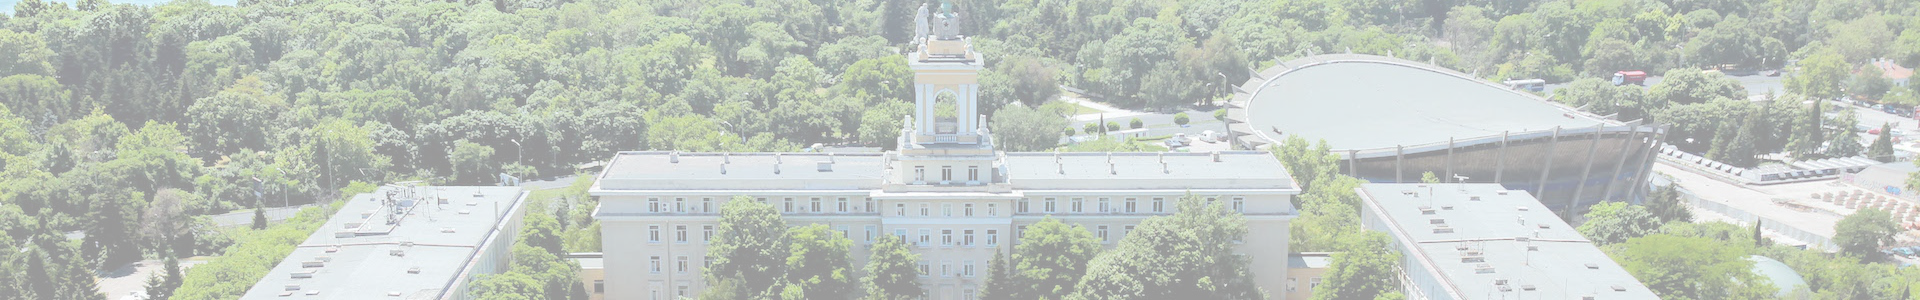
\includegraphics[width=370px, height=270px, trim=0 0 0 0px]{Snimka_MU_Varna_1.png}
}

\title[ \fontsize{5}{7}\selectfont Second International Scientific Conference Digital Transformation, Cyber Security and Resilience, September 30 - October 02, 2020, Varna, Bulgaria]{Cybersecurity in Donated Distributed Computing for Evolutionary Algorithms}

\author{Petar Tomov, Iliyan Zankinski,\\ Todor Balabanov\textsuperscript{0000-0003-3139-069X}}
%
% Bulgarian Academy of Sciences
% Institute of Information and Communication Technologies
% acad. Georgi Bonchev Str., block 2, office 514, 1113 Sofia, Bulgaria
% http://www.iict.bas.bg/
% iict@bas.bg
%

\date{30.IX-02.X.2020}

\institute[IICT-BAS, DIGILIENCE'20] {
	Institute of Information and Communication Technologies \\ 
	Bulgarian Academy of Sciences \\
	\medskip
	\textit{todorb@iinf.bas.bg}
}

\addtobeamertemplate{navigation symbols}{}{
    \usebeamerfont{footline}
    \usebeamercolor[fg]{footline}
    \hspace{1em}
    \insertframenumber/\inserttotalframenumber
}

\begin{document}

\begin{frame}
\titlepage
\end{frame}

\begin{frame}
\frametitle{Agenda}
\tableofcontents
\end{frame}

\section{Introduction}

\begin{frame}
\center \huge{Introduction}
\end{frame}

\subsection{}

\section{Conclusions}

\begin{frame}
\center \huge{Conclusions}
\end{frame}

\subsection{Advantages and Disadvantages}

\begin{frame}
\frametitle{Advantages}
\end{frame}

\begin{frame}
\frametitle{Disadvantages}
\end{frame}

\begin{frame}
\frametitle{Future Research}
\end{frame}

\subsection{Discussion}

\begin{frame}
\frametitle{Questions and Answers}
\center \huge{Thank you for your attention!}
\end{frame}

\end{document}
